\documentclass[12pt,a4paper]{article}
\usepackage[utf8]{inputenc}
\usepackage[T1]{fontenc}
\usepackage[english]{babel}
\usepackage{amsmath,amssymb,geometry,setspace,lmodern}
\usepackage{graphicx,float,caption,fancyhdr,listings,xcolor,booktabs,array}

\geometry{top=2cm,bottom=2cm,left=2.5cm,right=2.5cm}
\setstretch{1.3}
\pagestyle{fancy}\fancyhf{}\rfoot{\thepage}
\captionsetup[figure]{position=bottom,justification=centering}

\definecolor{codegray}{rgb}{0.95,0.95,0.95}
\definecolor{commentcolor}{rgb}{0.4,0.4,0.4}
\definecolor{keywordcolor}{rgb}{0.1,0.1,0.6}
\definecolor{stringcolor}{rgb}{0.2,0.5,0.2}
\lstset{
  language=Python, basicstyle=\ttfamily\scriptsize, backgroundcolor=\color{codegray},
  commentstyle=\color{commentcolor}\itshape, keywordstyle=\color{keywordcolor}\bfseries,
  stringstyle=\color{stringcolor}, frame=single, rulecolor=\color{black!30},
  showstringspaces=false, breaklines=true, columns=fullflexible, keepspaces=true
}
\newcommand{\code}[1]{\texttt{\small #1}}
\def\rowAlpha{A & B & C & D & E & F & G & H & I & J & K & L & M & N & O & P & Q & R & S & T & U & V & W & X & Y & Z}
\def\rowCnt{62 & 3 & 85 & 68 & 2 & 68 & 211 & 86 & 199 & 89 & 22 & 27 & 7 & 228 & 118 & 164 & 182 & 57 & 117 & 247 & 66 & 382 & 288 & 208 & 6 & 81}
\def\rowRankL{V & W & T & N & G & X & I & Q & P & O & S & J & H & C & Z & D & F & U & A & R & L & K & M & Y & B & E}
\def\rowRankN{382 & 288 & 247 & 228 & 211 & 208 & 199 & 182 & 164 & 118 & 117 & 89 & 86 & 85 & 81 & 68 & 68 & 66 & 62 & 57 & 27 & 22 & 7 & 6 & 3 & 2}

\def\keyPlain{a & b & c & d & e & f & g & h & i & j & k & l & m & n & o & p & q & r & s & t & u & v & w & x & y & z}
\def\keyCipher{T & A & H & O & V & C & J & Q & X & E & L & S & Z & G & N & U & B & I & P & W & D & K & R & Y & F & M}


\begin{document}

\begin{titlepage}
\begin{center}
  \textbf{MINISTERUL EDUCAȚIEI ȘI CERCETĂRII}\\
  \textbf{AL REPUBLICII MOLDOVA}\\[0.5em]
  \textbf{UNIVERSITATEA TEHNICĂ A MOLDOVEI}\\
  \textbf{Facultatea Calculatoare, Informatică și Microelectronică}\\
  \textbf{Departamentul Ingineria Software și Automatică}\\[2em]

  \vspace{1.5cm}
  \textbf{\Large Tacu Igor \textemdash{} FAF-242}\\[3em]

  \textbf{\Large RAPORT}\\[0.5em]
  Lucrare de laborator nr.\ 2\\[0.5em]
  \textbf{Criptografie}\\[0.5em]
  \textbf{Criptanaliza cifrurilor monoalfabetice}\\[0.5em]
  Varianta 23\\[3em]

  \vfill
  \begin{flushright}
    Lector:\\
    Maia Zaica\\
    DISA, FCIM, UTM
  \end{flushright}
  \vfill

  \large \textbf{Chișinău \textemdash{} 2026}
\end{center}
\end{titlepage}

\tableofcontents
\newpage

% ============================================================
\section{Sarcina lucrării}

Se interceptează un mesaj criptat cu un cifru monoalfabetic despre care se știe că
textul clar este scris în limba engleză. Folosind analiza frecvenței literelor trebuie
găsit mesajul original. Doar literele au fost criptate; spațiile, cifrele și
semnele de punctuație au rămas necriptate. Fiecare student primește varianta
corespunzătoare numărului său de ordine din lista grupei; numărul meu este 23, deci
lucrez cu criptograma \textbf{V23}.

% ============================================================
\section{Teorie scurtă}

Într-un cifru monoalfabetic fiecare literă a textului clar este înlocuită întotdeauna
cu aceeași literă a textului criptat, adică cheia este o permutare a alfabetului. Pentru
alfabetul englez de 26 de litere există $26! \approx 4{,}03\cdot10^{26}$ chei, deci o căutare
exhaustivă nu este posibilă. Totuși, punctul slab este că \emph{frecvența de apariție a
literelor se păstrează}: dacă un text este suficient de lung, cea mai frecventă literă din
criptogramă corespunde, cu mare probabilitate, celei mai frecvente litere a limbii
(în engleză E, apoi T, A, O, I, N, \dots, vezi tabelul 2.2 din îndrumar).

Frecvențele singure nu ajung, deoarece un text concret nu respectă exact tabelul.
De aceea se folosesc și alte „trăsături de personalitate” ale limbii:
\begin{itemize}
  \item digrafele frecvente: TH, HE, AN, IN, ER, ON, RE, ED, ND, HA, AT, EN;
  \item trigrafele frecvente: THE, AND, THA, ENT, ION, TIO, FOR, NDE, HAS, NCE;
  \item literele dublate (SS, EE, TT, OO, FF) și cuvintele dintr-o singură literă (A, I);
  \item cuvinte frecvente care apar pe măsură ce se fac înlocuiri (de exemplu T\texttt{*}E $\to$ THE).
\end{itemize}
Procesul este iterativ și necesită decizii ale omului: se fixează cele mai sigure
înlocuiri, se citește textul parțial decriptat și se corectează ipotezele.

% ============================================================
\section{Criptograma interceptată (varianta 23)}

Criptograma conține \textbf{3073 de litere} (fișierul \code{lab2/cipher\_v23.txt}). Începutul ei:
\begin{lstlisting}[language={}]
Cixvoztg oxo pnzv jvgvwxhp rnil cni qxz, adw, avhtdpv qv rtp qtgofrxwq t htzvit, qv qvsuvo wqv
hifuwnsnjxpwp rqn rviv snnlxgj cni Athng'phxuqvi pxjgtwdivp xg Pqtlvpuvtiv af ztlxgj uqnwnjituqxh
vgstijvzvgwpnc wqv Vsxmtavwqtg uixgwxgj wqtw cxjdivo xg wqv rnil. Wqv Ovutiwzvgw
\end{lstlisting}

% ============================================================
\section{Atacul prin analiza frecvențelor}

\subsection{Frecvențele literelor din criptogramă}

Pentru calculul frecvențelor am scris un mic program (\code{lab2/freq.py}):
\begin{lstlisting}
def letters(text):
    return [c for c in text.upper() if c in ABC]

def letter_freq(text):
    return Counter(letters(text))
\end{lstlisting}
Funcția \code{letters} păstrează doar literele (ignoră spațiile, cifrele și punctuația),
iar \code{letter\_freq} numără apariția fiecăreia. Rezultatul este în tabelul 1, ordonat
alfabetic, și în tabelul 2, ordonat descrescător.

\begin{table}[H]
\centering\scriptsize\setlength{\tabcolsep}{2.3pt}
\begin{tabular}{@{}l*{26}{c}@{}}
\toprule
Litera & \rowAlpha \\
Frecvența & \rowCnt \\
\bottomrule
\end{tabular}
\caption{Frecvența literelor în criptograma interceptată (număr de apariții).}
\end{table}

\begin{table}[H]
\centering\scriptsize\setlength{\tabcolsep}{2.3pt}
\begin{tabular}{@{}l*{26}{c}@{}}
\toprule
Litera & \rowRankL \\
Frecvența & \rowRankN \\
\bottomrule
\end{tabular}
\caption{Aceleași frecvențe, în ordine descrescătoare.}
\end{table}

\begin{figure}[H]
\centering
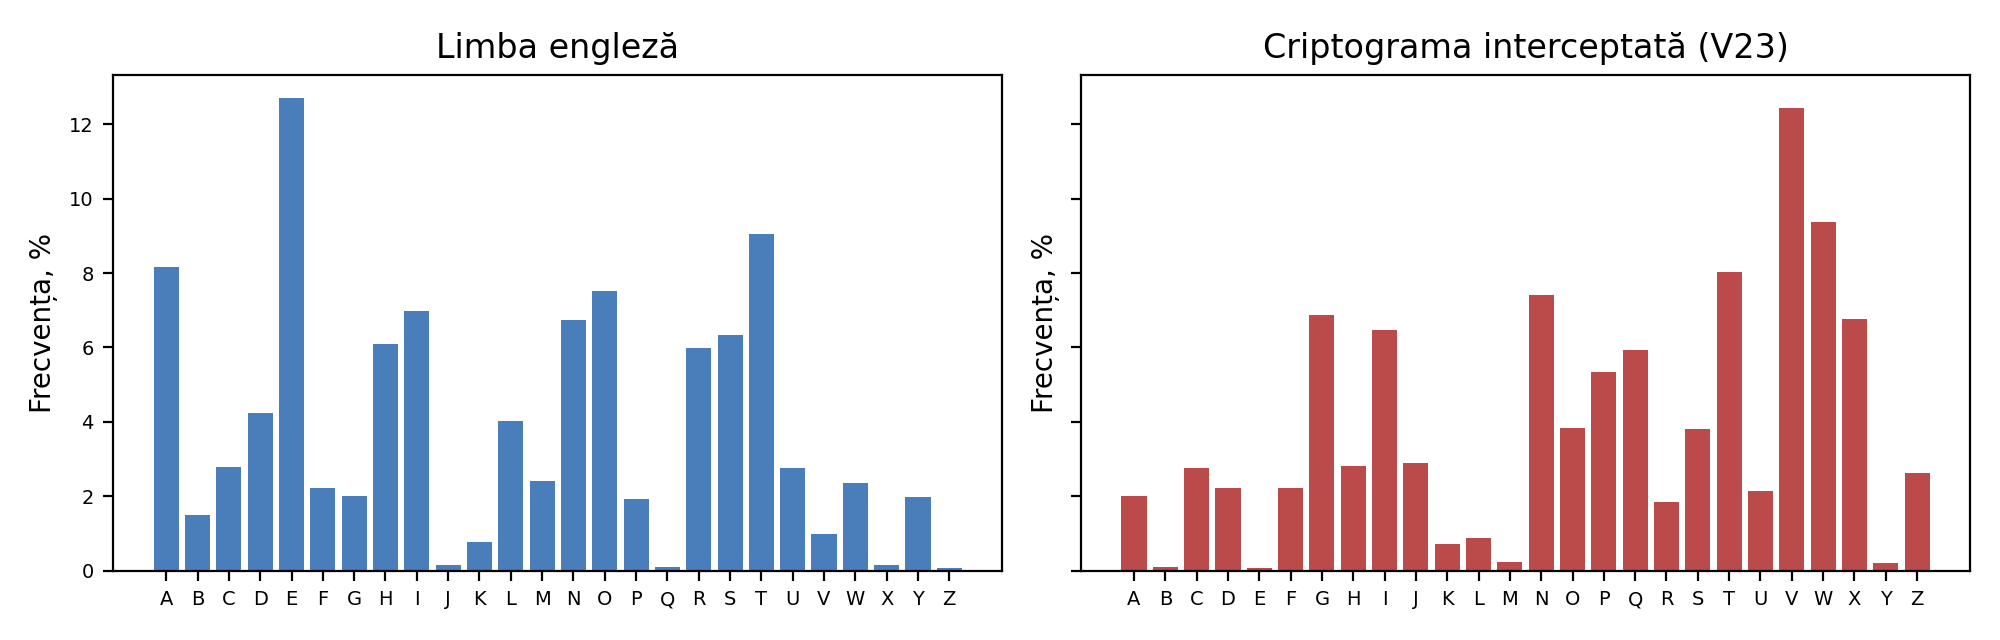
\includegraphics[width=\textwidth]{images/freq_compare.png}
\caption{Frecvența literelor în limba engleză (stânga) și în mesajul interceptat (dreapta).}
\end{figure}

Cele mai frecvente litere în engleză sunt, în ordine, \texttt{E T A O I N S H R D L C U M W F G Y P B V K J X Q Z},
iar în criptogramă \texttt{V W T N G X I Q P O S J H C Z D F U A R L K M Y B E}. Cele două ordini sunt
destul de apropiate la început (V--E, W--T, T--A, N--O, G--N, X--I), dar nu identice, deci
trebuie verificat fiecare pas. Cele mai frecvente trigrame ale criptogramei sunt
\texttt{WQV} (65 de apariții), \texttt{TGO} (20), \texttt{XGJ} (18), \texttt{QVI} (17), iar cele mai frecvente
cuvinte \texttt{WQV} (41), \texttt{NC} (31), \texttt{XG} (16), \texttt{TGO} (15), \texttt{T} (14).

\subsection{Substituțiile pas cu pas}

Mai jos, literele deja descifrate sunt scrise cu litere mici, iar cele necunoscute cu
litere mari (ca în exemplul din îndrumar). Pentru fiecare pas se afișează primele 5 rânduri
ale mesajului.

\paragraph{Pasul 1: V=e, W=t.} V și W sunt cele mai frecvente litere, ca E și T în engleză.
\begin{lstlisting}[language={}]
CIXeOZTG OXO PNZe JeGetXHP RNIL CNI QXZ, ADt, AeHTDPe Qe RTP QTGOFRXtQ T HTZeIT, Qe QeSU
HIFUtNSNJXPtP RQN ReIe SNNLXGJ CNI ATHNG'PHXUQeI PXJGTtDIeP XG PQTLePUeTIe AF ZTLXGJ UQN
eGSTIJeZeGtPNC tQe eSXMTAetQTG UIXGtXGJ tQTt CXJDIeO XG tQe RNIL. tQe OeUTItZeGt
NCHXUQeIP NC tQe IXKeIATGL STANITtNIXeP HNGPXPteO NC 14 NI 15 QXJQ-PHQNNSTGO HNSSeJe JIT
RQN TPPXJGeO tQe XGOXKXODTS SetteIP XG tQePeeSXMTAetQTG teYtP tN NGe NI tQe NtQeI NC tRN
\end{lstlisting}

\paragraph{Pasul 2: Q=h.} trigrama cea mai frecventă, WQV, este aproape sigur THE, deci Q = h.
\begin{lstlisting}[language={}]
CIXeOZTG OXO PNZe JeGetXHP RNIL CNI hXZ, ADt, AeHTDPe he RTP hTGOFRXth T HTZeIT, he heSU
HIFUtNSNJXPtP RhN ReIe SNNLXGJ CNI ATHNG'PHXUheI PXJGTtDIeP XG PhTLePUeTIe AF ZTLXGJ UhN
eGSTIJeZeGtPNC the eSXMTAethTG UIXGtXGJ thTt CXJDIeO XG the RNIL. the OeUTItZeGt
NCHXUheIP NC the IXKeIATGL STANITtNIXeP HNGPXPteO NC 14 NI 15 hXJh-PHhNNSTGO HNSSeJe JIT
RhN TPPXJGeO the XGOXKXODTS SetteIP XG thePeeSXMTAethTG teYtP tN NGe NI the NtheI NC tRN
\end{lstlisting}

\paragraph{Pasul 3: T=a, G=n, O=d.} TGO (trigramă frecventă, cuvânt de 3 litere) este AND.
\begin{lstlisting}[language={}]
CIXedZan dXd PNZe JenetXHP RNIL CNI hXZ, ADt, AeHaDPe he RaP handFRXth a HaZeIa, he heSU
HIFUtNSNJXPtP RhN ReIe SNNLXnJ CNI AaHNn'PHXUheI PXJnatDIeP Xn PhaLePUeaIe AF ZaLXnJ UhN
enSaIJeZentPNC the eSXMaAethan UIXntXnJ that CXJDIed Xn the RNIL. the deUaItZent
NCHXUheIP NC the IXKeIAanL SaANIatNIXeP HNnPXPted NC 14 NI 15 hXJh-PHhNNSand HNSSeJe JIa
RhN aPPXJned the XndXKXdDaS SetteIP Xn thePeeSXMaAethan teYtP tN Nne NI the NtheI NC tRN
\end{lstlisting}

\paragraph{Pasul 4: N=o, C=f.} NC este cuvântul de două litere OF (N a mai apărut în WN = to).
\begin{lstlisting}[language={}]
fIXedZan dXd PoZe JenetXHP RoIL foI hXZ, ADt, AeHaDPe he RaP handFRXth a HaZeIa, he heSU
HIFUtoSoJXPtP Rho ReIe SooLXnJ foI AaHon'PHXUheI PXJnatDIeP Xn PhaLePUeaIe AF ZaLXnJ Uho
enSaIJeZentPof the eSXMaAethan UIXntXnJ that fXJDIed Xn the RoIL. the deUaItZent
ofHXUheIP of the IXKeIAanL SaAoIatoIXeP HonPXPted of 14 oI 15 hXJh-PHhooSand HoSSeJe JIa
Rho aPPXJned the XndXKXdDaS SetteIP Xn thePeeSXMaAethan teYtP to one oI the otheI of tRo
\end{lstlisting}

\paragraph{Pasul 5: X=i.} XG este cuvântul IN (G = n deja cunoscut).
\begin{lstlisting}[language={}]
fIiedZan did PoZe JenetiHP RoIL foI hiZ, ADt, AeHaDPe he RaP handFRith a HaZeIa, he heSU
HIFUtoSoJiPtP Rho ReIe SooLinJ foI AaHon'PHiUheI PiJnatDIeP in PhaLePUeaIe AF ZaLinJ Uho
enSaIJeZentPof the eSiMaAethan UIintinJ that fiJDIed in the RoIL. the deUaItZent
ofHiUheIP of the IiKeIAanL SaAoIatoIieP HonPiPted of 14 oI 15 hiJh-PHhooSand HoSSeJe JIa
Rho aPPiJned the indiKidDaS SetteIP in thePeeSiMaAethan teYtP to one oI the otheI of tRo
\end{lstlisting}

\paragraph{Pasul 6: R=w, P=s.} RTP = WAS, RQN = WHO, RVIV = WERE, după ce T, Q, V sunt cunoscute.
\begin{lstlisting}[language={}]
fIiedZan did soZe JenetiHs woIL foI hiZ, ADt, AeHaDse he was handFwith a HaZeIa, he heSU
HIFUtoSoJists who weIe SooLinJ foI AaHon'sHiUheI siJnatDIes in shaLesUeaIe AF ZaLinJ Uho
enSaIJeZentsof the eSiMaAethan UIintinJ that fiJDIed in the woIL. the deUaItZent
ofHiUheIs of the IiKeIAanL SaAoIatoIies Honsisted of 14 oI 15 hiJh-sHhooSand HoSSeJe JIa
who assiJned the indiKidDaS SetteIs in theseeSiMaAethan teYts to one oI the otheI of two
\end{lstlisting}

\paragraph{Pasul 7: I=r.} CNI = FOR (I este ultima literă a cuvântului).
\begin{lstlisting}[language={}]
friedZan did soZe JenetiHs worL for hiZ, ADt, AeHaDse he was handFwith a HaZera, he heSU
HrFUtoSoJists who were SooLinJ for AaHon'sHiUher siJnatDres in shaLesUeare AF ZaLinJ Uho
enSarJeZentsof the eSiMaAethan UrintinJ that fiJDred in the worL. the deUartZent
ofHiUhers of the riKerAanL SaAoratories Honsisted of 14 or 15 hiJh-sHhooSand HoSSeJe Jra
who assiJned the indiKidDaS Setters in theseeSiMaAethan teYts to one or the other of two
\end{lstlisting}

\paragraph{Pasul 8: J=g.} trigrama XGJ = ING.
\begin{lstlisting}[language={}]
friedZan did soZe genetiHs worL for hiZ, ADt, AeHaDse he was handFwith a HaZera, he heSU
HrFUtoSogists who were SooLing for AaHon'sHiUher signatDres in shaLesUeare AF ZaLing Uho
enSargeZentsof the eSiMaAethan Urinting that figDred in the worL. the deUartZent
ofHiUhers of the riKerAanL SaAoratories Honsisted of 14 or 15 high-sHhooSand HoSSege gra
who assigned the indiKidDaS Setters in theseeSiMaAethan teYts to one or the other of two
\end{lstlisting}

\paragraph{Pasul 9: H=c, F=y, U=p, S=l.} HIFUWNSNJF = CRYPTOLOGY, găsit după șablonul c-r-y-p-t-o-l-o-g-y.
\begin{lstlisting}[language={}]
friedZan did soZe genetics worL for hiZ, ADt, AecaDse he was handywith a caZera, he help
cryptologists who were looLing for Aacon'scipher signatDres in shaLespeare Ay ZaLing pho
enlargeZentsof the eliMaAethan printing that figDred in the worL. the departZent
ofciphers of the riKerAanL laAoratories consisted of 14 or 15 high-schooland college gra
who assigned the indiKidDal letters in theseeliMaAethan teYts to one or the other of two
\end{lstlisting}

\paragraph{Pasul 10: Z=m.} ZTG = MAN.
\begin{lstlisting}[language={}]
friedman did some genetics worL for him, ADt, AecaDse he was handywith a camera, he help
cryptologists who were looLing for Aacon'scipher signatDres in shaLespeare Ay maLing pho
enlargementsof the eliMaAethan printing that figDred in the worL. the department
ofciphers of the riKerAanL laAoratories consisted of 14 or 15 high-schooland college gra
who assigned the indiKidDal letters in theseeliMaAethan teYts to one or the other of two
\end{lstlisting}

\paragraph{Pasul 11: A=b, D=u.} Athng = BACON, ndwsvw = OUTLET.
\begin{lstlisting}[language={}]
friedman did some genetics worL for him, but, because he was handywith a camera, he help
cryptologists who were looLing for bacon'scipher signatures in shaLespeare by maLing pho
enlargementsof the eliMabethan printing that figured in the worL. the department
ofciphers of the riKerbanL laboratories consisted of 14 or 15 high-schooland college gra
who assigned the indiKidual letters in theseeliMabethan teYts to one or the other of two
\end{lstlisting}

\paragraph{Pasul 12: L=k, M=z.} Pqtlvpuvtiv = SHAKESPEARE, Vsxmtavwq = ELIZABETH.
\begin{lstlisting}[language={}]
friedman did some genetics work for him, but, because he was handywith a camera, he help
cryptologists who were looking for bacon'scipher signatures in shakespeare by making pho
enlargementsof the elizabethan printing that figured in the work. the department
ofciphers of the riKerbank laboratories consisted of 14 or 15 high-schooland college gra
who assigned the indiKidual letters in theseelizabethan teYts to one or the other of two
\end{lstlisting}

\paragraph{Pasul 13: K=v, B=q, Y=x, E=j.} Kxijxg = VIRGIN, bdxhl = QUICK, „4 Y 7” = 4 x 7, Enqg = JOHN.
\begin{lstlisting}[language={}]
friedman did some genetics work for him, but, because he was handywith a camera, he help
cryptologists who were looking for bacon'scipher signatures in shakespeare by making pho
enlargementsof the elizabethan printing that figured in the work. the department
ofciphers of the riverbank laboratories consisted of 14 or 15 high-schooland college gra
who assigned the individual letters in theseelizabethan texts to one or the other of two
\end{lstlisting}


\subsection{Mesajul descifrat}

Rezultatul final este (fiecare literă a criptogramei a fost înlocuită; cratimele lungi
sunt scrise „--”):

\begin{lstlisting}[language={}]
friedman did some genetics work for him, but, because he was handywith a camera, he helped
the cryptologists who were looking for bacon'scipher signatures in shakespeare by making
photographic enlargementsof the elizabethan printing that figured in the work. the
department ofciphers of the riverbank laboratories consisted of 14 or 15 high-schooland
college graduates who assigned the individual letters in theseelizabethan texts to one or
the other of two fonts of type as part of thebaconian search. fabyan gave them their living
plus a salary of about$50 a month. the staff was fed and housed in engledew and
hoovercottages, the cipher laboratories taking up the first floor of engledew.the young
woman who collated the work of many of the other staffmembers was elizebeth smith. she had
been , born august 26, 1892, inhuntington, indiana, the youngest of the nine children of
john m. smith,a dairyman, banker, and county republican committeeman, and hiswife, sopha,
who spelled her daughter's christian name witb an einstead of an a in the middle because she
was not going to have anyonecalling her child "eliza." after completing high school in
huntington,elizebeth attended wooster college briefly but was graduated fromhillsdale
college in michigan where she had majored in english. whileworking at the newberry library
in chicago, she was recruited byfabyan and began work there in 1916.neither she nor friedman
had given any particular previous thoughtto cryptology, but they began to get personally
interested in the work. itis yet another of the ironies of cryptologic history that the
interest of twoforemost cryptologists was aroused by a false doctrine--a doctrine,moreover,
against which they later were to wage a lifetime battle. for attable at the riverbank
cottages they heard gaudy tales of lustyelizabethan life, of the not-so-virgin queen, of
courtiers' intrigues andthe secret histories of the great names of english history--all
actuallyinvalid decipherments of shakespeare's plays tending to prove thatbacon had written
them, related by the gentle, upright, but self-deludedwoman who had "deciphered" them, mrs.
elizabeth wells gallup. thesestories stirred friedman's dormant interest; he began to do
some of thecryptology, and inevitably its puissant magic seeped like the fume ofpoppies into
his mind and spirit and intoxicated him."when it came to the cryptology," he recalled years
later,"something in me found an outlet."an understatement. he soon found himself head of the
department ofciphers as well as the department of genetics at riverbank. theattraction he
felt for cryptology was reinforced by the attraction he felt fora cryptologist: the quick-
witted and sprightly miss smith. in may of 1917they were married and started the most famous
husband-and-wife teamin the history of cryptology.america had declared war a month before,
and river-bank, which hadthe only going cryptologic concern in the country, began getting,
on aninformal basis, cryptograms for solution from various governmentbureaus. probably the
most important were messages to and from a ringof 125 hindus who, with german aid, were
taking advantage ofengland's preoccupation in europe to strike for indian independence.the
intercepts were given to friedman for solution, and he quickly solvedthe number cipher used
in cablegrams to berlin. the letters of theplaintext and of the keyword were transformed
into digits by means of a4 x 7 checkerboard with a normal alphabet;  the key digits were
thenadded to those of the plaintext to form the ciphertext. one key waslamp. each agent had
his own key, but friedman had no trouble insolving them. nor was he stumped by a system
usually regarded byamateurs as the ne plus ultra of cryptographic security: a book cipher.
\end{lstlisting}


Mici greșeli de ortografie și spații lipsă (de exemplu „handywith”, „witb an einstead”)
provin din criptograma dată, nu din atac: spațiile și punctuația rămân necriptate, iar
pentru acele cuvinte nu există o altă citire a literelor.

\subsection{Cheia reconstituită}

Din substituțiile găsite se reconstituie alfabetul de criptare (tabelul 3). Cheia este o
permutare completă a celor 26 de litere, ceea ce confirmă corectitudinea atacului.

\begin{table}[H]
\centering\scriptsize\setlength{\tabcolsep}{2.3pt}
\begin{tabular}{@{}l*{26}{c}@{}}
\toprule
Alfabet clar & \keyPlain \\
Alfabet criptat & \keyCipher \\
\bottomrule
\end{tabular}
\caption{Alfabetul reconstituit al mesajului criptat (varianta 23).}
\end{table}

% ============================================================
\section{Implementare}

Programele sunt în Python 3, fără biblioteci externe (în afară de \code{matplotlib} pentru grafic):
\code{freq.py} (frecvențe, digrame, trigrame, aplicarea cheii), \code{attack.py} (lista
substituțiilor cu justificarea fiecăreia) și \code{make\_report\_data.py} (generează graficul
și fragmentele din acest raport).
\begin{lstlisting}
def apply(text, mapping):
    # litere cunoscute -> mici, necunoscute -> mari, restul neschimbat
    return "".join(mapping.get(c.upper(), c.upper()) if c.isalpha() else c
                   for c in text)
\end{lstlisting}
Funcția \code{apply} înlocuiește fiecare literă cu corespondentul din dicționarul
\code{mapping} (literă criptată $\to$ literă clară) și lasă neschimbate caracterele care nu sunt litere.
Atacul în sine este un lanț de ipoteze verificate vizual pe textul parțial decriptat; la final
\code{make\_report\_data.py} verifică (\code{assert}) că cheia obținută este o permutare a alfabetului.

% ============================================================
\section{Concluzii}

Cifrul monoalfabetic poate avea un spațiu al cheilor imens ($26!$), dar nu este sigur:
pentru o criptogramă de numai 3073 de litere au fost suficiente frecvențele literelor,
trigrama \texttt{THE}, cuvintele scurte frecvente (\texttt{AND, OF, IN, TO, WAS}) și recunoașterea
unor cuvinte mai lungi (\texttt{CRYPTOLOGY, SHAKESPEARE, ELIZABETH}) pentru a recupera integral
textul și cheia. Cele mai multe litere (E, T, A, O, N, I, S, H, R) au fost identificate din
frecvențe și trigrame, iar literele rare (J, Q, X, Z, K, V, B) abia la sfârșit, din context,
pentru că frecvența lor este prea mică pentru a fi statistic de încredere. Atacul nu poate fi
făcut complet automat: sunt necesare cunoștințe despre limbă, iar pașii s-au verificat citind
textul parțial descifrat. Concluzia este că un cifru bun trebuie să ascundă frecvențele
(de exemplu prin substituție polialfabetică), nu doar să aibă multe chei.

% ============================================================
\section{Codul sursă}

Codul complet (folderul \texttt{lab2}) este disponibil în depozitul GitHub:\\
\texttt{https://github.com/igortacu/criptography}

\end{document}
